\chapter{Evaluation}
\label{chp:evaluation}

\section{Controlled Movements}
\label{sec:controlled_movements}

% Comparison deadreckoning accuracy of battery powered robot with solar powered robot

% Try at least one more supercapacitor: 10mF
% Study reducing the frequency of power interrupts ie smaller energy buffer.
% How does this effect the accuracy of locomotion?
% Can the frequency of power interrupts be related to the 

% Video of robot movement

In this section the accuracy of movement of the battery-less robot is evaluated and compared to its battery powered counterpart.

\subsection{Experimental setup}

To be able to compare the accuracy of the robot while it is exposed to increasingly smaller on times, a variety of movements is recorded using an overhead camera.
A stand with a Nikon D610 DSLR camera is positioned on a tabletop, as seen in Figure \ref{fig:movement_setup}.
The corners of a square of 80$\times$80\,cm are indicated with black corner markers.
This square is used as a reference to convert the robots movement from pixels to cm.
Two movements are compared: (1) the robot preforms a straight movement of 75\,cm and (2) the robot preforms a circular movement of 360 degrees with a radius of 30\,cm.

\begin{figure}
	\centering
	\begin{subfigure}[b]{0.45\textwidth}
		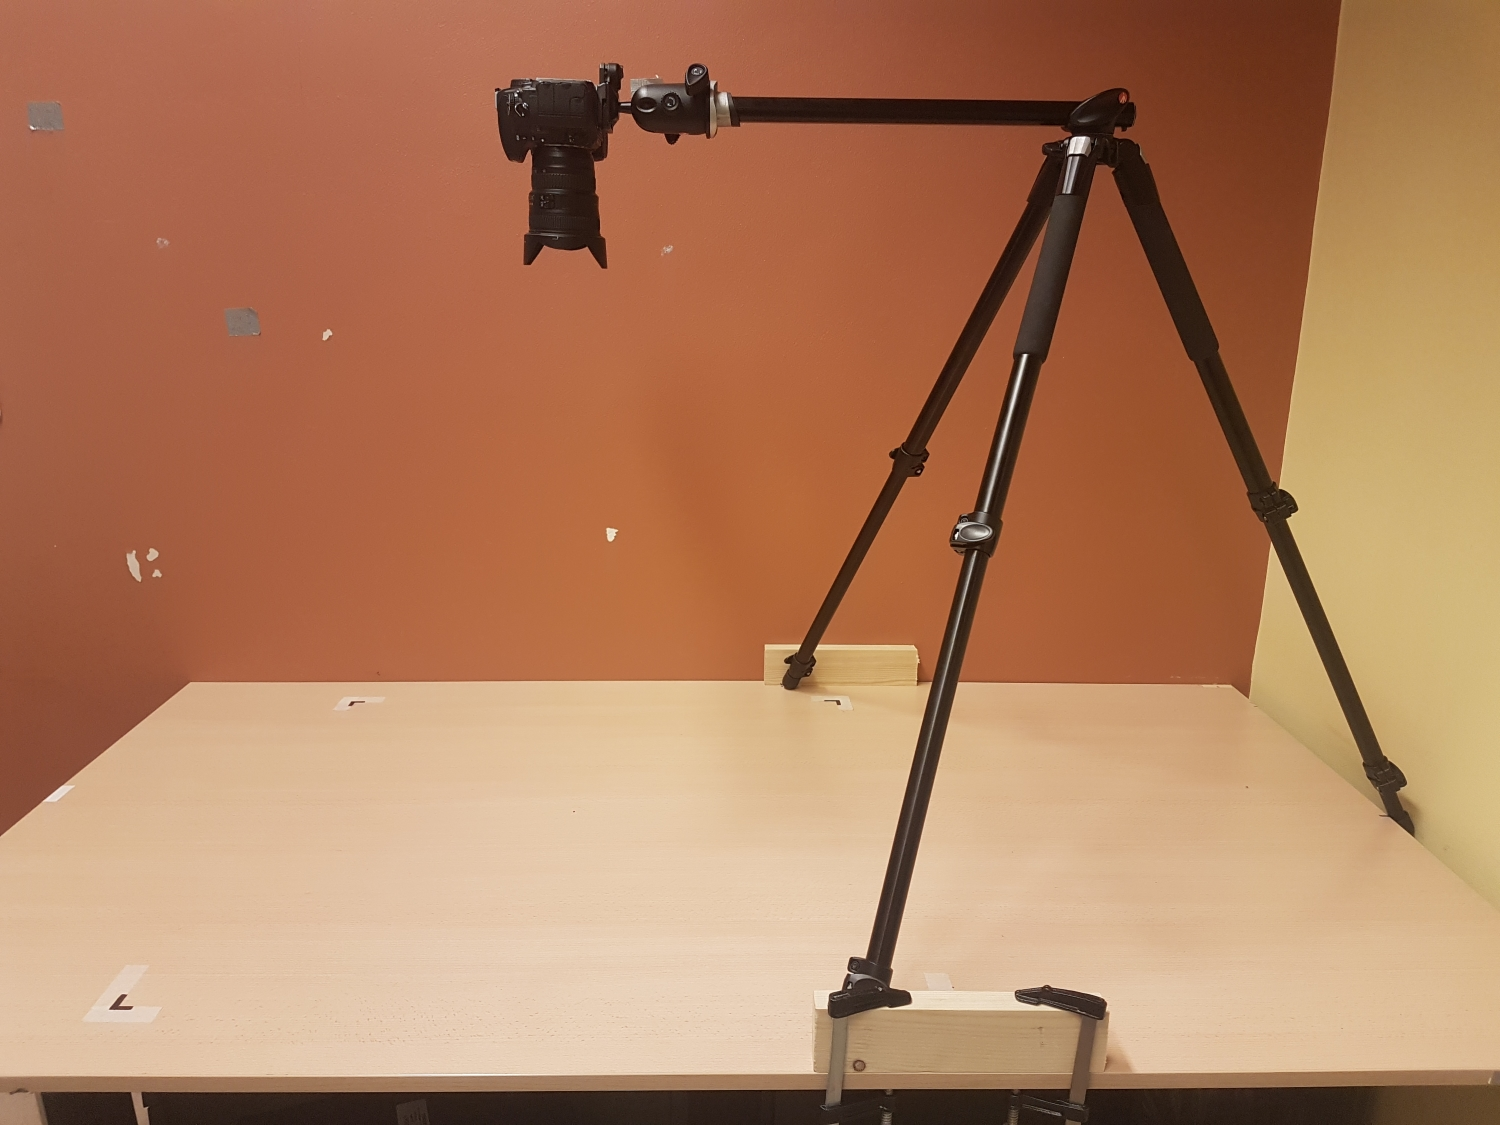
\includegraphics[width=\textwidth]{pics/movement_setup.jpg}
		\caption{Camera setup}
		\label{fig:movement_setup}
	\end{subfigure}
	\quad
	\begin{subfigure}[b]{0.45\textwidth}
		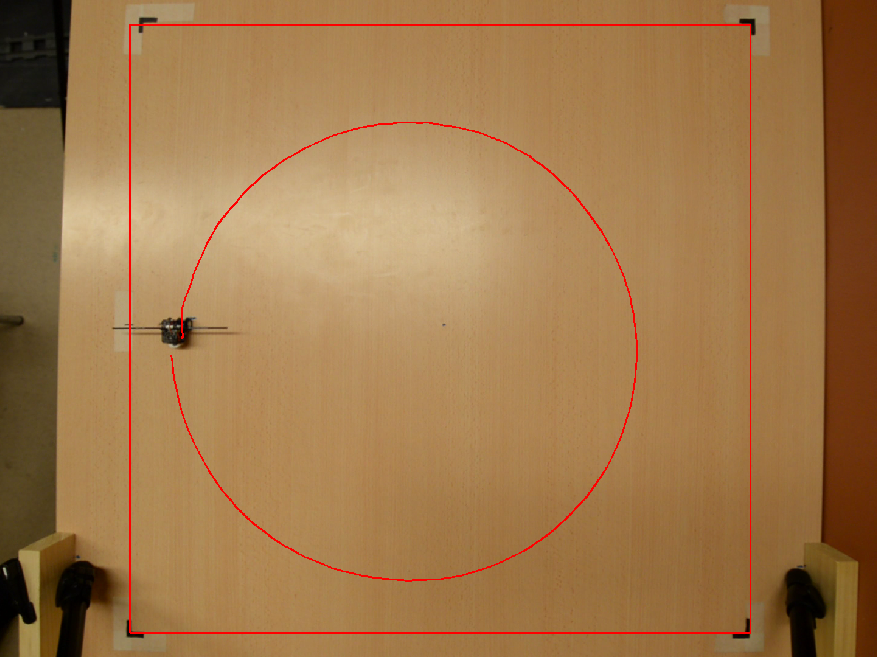
\includegraphics[width=\textwidth]{pics/movement_example.png}
		\caption{Tracking with OpenCV}
		\label{fig:movement_example}
	\end{subfigure}
	\caption{Experimental setup to record the robots movement.}
\end{figure}

\subsubsection{Tracking the Movement}

%The robot is programmed to perform the movement at a desired PWM target ie at a specified speed, and optional on time.
Before the robot executes the movement, a green marker is placed on top of the robot.
The marker is the reference point that is used by the tracking software.
The camera is used to record the movement, which then is analyzed using Python and OpenCV 3.2.
An example of a tracked movement can be seen in Figure \ref{fig:movement_example}.
The red square is drawn using OpenCV and visually sized to fit the square marked by the black corner markings on the table top.
Because the size of the square is known to be 80$\times$80\,cm, the movement coordinates can be converted from pixels to centimeter.

\subsubsection{Target Duty Cycle}
To evaluate the influence of speed on the movement accuracy, each movement is executed at three different target duty cycle settings: 40\%, 65\% and 90\% of the maximum duty cycle.
The highest setting is chosen to be equal to 90\,\% because it allows the PID controller to also increase the target duty cycle.
If the target duty cycle is set to a 100\,\% the controller is only able to decrease the speed of the faster rotating motor because the maximum motor speed is bounded at a 100\,\%.


\subsubsection{Power Interrupts}

The on time is determined by the energy stored in the capacitor and the power consumed by the robot for movement.
To evaluate different on times, besides the one created with the 22\,mF supercapacitor, additional power interrupts are generated artificially.
The power interrupts, i.e. the capacitor running out of energy, are created artificially using a timer that resets the MCU.
If the interrupts are generated artificially, the robot is powered from a battery.
The MSP430FR5969 has the functionality to enable a brownout reset through software, which is used to simulate the event of the supply voltage dropping below the required operating voltage~\cite{msp430fr_family_guide_2017}.
A timer is used to generate the power interrupt after a predefined time.

\subsubsection{On Time}

With the selected capacitor of 22\,mF, the robot can operate around 1 second. 
To find the minimal on time that is required to allow control the robot, it is programmed to perform a four second straight movement.
The movement is recorded for each target duty cycle and the on times of 0.4\,s, 0.3\,s and 0.2\,s are evaluated.

The results in Figure \ref{fig:decreasing_power_period} show that for the higher duty cycle targets an on time of 0.3\,s leads to significant drift to one side, which is classified as uncontrolled behavior.
The control loop was not able to stabilize the movement before a power interrupt occurs, and therefore the robot drifts to the side of its weakest motor.
The duration that power is available might not be long enough for the motors to reach their steady state speed, making linear control of the motors impossible.
Increasing the target duty cycle shows that a longer on time is required to control the movement. 
Therefore, the on times evaluated in this experiment are set to 1.0\,s and 0.5\,s.


\begin{figure}
	\begin{subfigure}[b]{0.32\textwidth}
		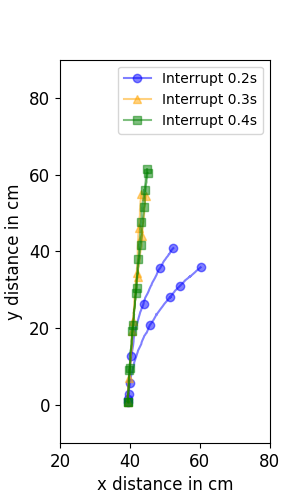
\includegraphics[width=\textwidth]{pics/figure_40.png}
		\caption{Target 40\%}
		\label{fig:target_40}
	\end{subfigure}
	\begin{subfigure}[b]{0.32\textwidth}
		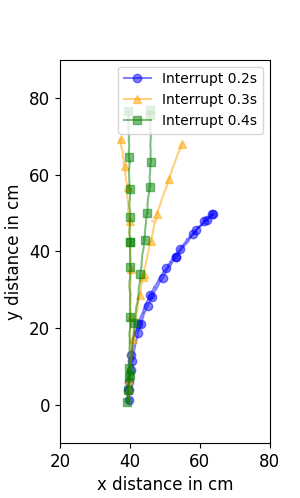
\includegraphics[width=\textwidth]{pics/figure_65.png}
		\caption{Target 65\%}
		\label{fig:target_65}
	\end{subfigure}
	\begin{subfigure}[b]{0.32\textwidth}
		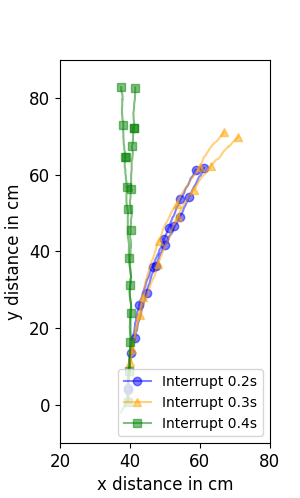
\includegraphics[width=\textwidth]{pics/figure_90.png}
		\caption{Target 90\%}
		\label{fig:target_90}
	\end{subfigure}
	\caption{Accuracy of straight movements while the on time is decreased, for each target duty cycle.}
	\label{fig:decreasing_power_period}
\end{figure}

\subsubsection{Speed Calibration}
Another thing that can be observed from the results in Figure \ref{fig:decreasing_power_period}, is the distance covered by the robot decreases by decreasing the target and/or on time.
Without any sensors or external feedback of the robots speed, it is difficult to determine the distance that the robot has traveled.
A rough speed estimate allows the robot to stay within the view of the camera.
The average speed is estimated for each target duty cycle and one time combination.
This is achieved by first determining the time that the robot requires to move approximately 150\,cm for each target duty cycle without power interrupts.
When the robot experiences power interrupts, the average speed of an active period becomes lower due to frequent acceleration from a standstill.
Therefore, power interrupts increase the runtime required to make the robot travel approximately the same distance.

Finally, the average of five complete movement measurements is computed and divided by the commanded runtime of the robot to acquire an average speed for each combination, as seen from Table \ref{tab:val_calib}.


\begin{table}[t]
	\centering
	\small
	\caption{The calibrated speeds in centimeter per second for each target duty cycle and on time combination.}
	\label{tab:val_calib}
	\begin{tabular}{|l||l|l|l|l|l|l|}
		\hline
		Target (\%) & No interrupt & 1.0\,s & 0.5\,s & Solar \\
		\hline \hline
		 40 & 18.9 & 18.0 & 15.9 & 16.0\\
	     65 & 24.0 & 21.3 & 18.8 & 20.8\\
		 90 & 28.8 & 25.7 & 22.7 & 23.3\\
		\hline
	\end{tabular}
\end{table}

%\begin{table}[t]
%	\centering
%	\small
%	\caption{The calibrated speeds.}
%	\label{tab:val_calib}
%	\begin{tabular}{|l|l||l|l|l|l|l|l|}
%		\hline
%		Target (\%) & & No int & 1.25\,s & 1.0\,s & 0.75\,s & 0.5\,s & Solar \\
%		\hline \hline
%		40 & cm/s & 18.9 & 18.2 & 18.0 & 17.1 & 15.9 & 16.0\\
%		65 & cm/s & 24.0 & 22.2 & 21.3 & 20.8 & 18.8 & 20.8\\
%		90 & cm/s & 28.8  & 26.4 & 25.7 & 24.5 & 22.7 & 23.3 \\
%		\hline
%	\end{tabular}
%\end{table}

\subsection{Straight Movements}
\label{eval:straight_movements}

Using the calibrated speeds and selected on times, the robot is commanded to perform a straight movement of 75\,cm from position (40,0) cm within the reference frame.
Each combination is recorded multiple times and the motion data is extracted from the video using Python and OpenCV.
The results in Figure \ref{fig:straight_movements} show that the distance traveled by the robot, for each measurement, approximates the commanded 75\,cm.
Additionally, the results show a varying horizontal deviation between the start and end point.
The horizontal deviation may be a consequence of inaccuracy in performing the movement.
However, it is more likely that the error originates from in the start position of the robot, because the robot is expected to not be positioned exactly perpendicular to the reference frame of 80$\times$80\,cm.
Even though the robot is positioned carefully in the same start position, it is inevitable the start angle is not exactly equal to other measurements.

\begin{figure}
	\centering
	\begin{subfigure}[b]{0.32\textwidth}
		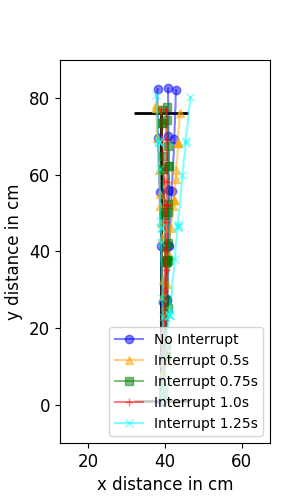
\includegraphics[width=\textwidth]{pics/straight_40.png}
		\caption{Target 40\%}
		\label{fig:stra_exp1}
	\end{subfigure}
	\begin{subfigure}[b]{0.32\textwidth}
		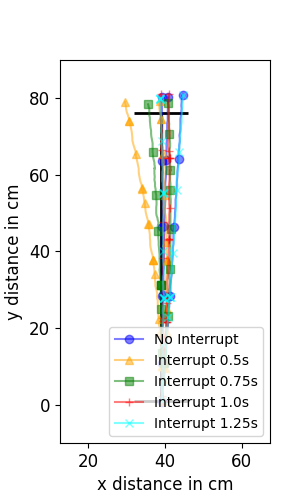
\includegraphics[width=\textwidth]{pics/straight_65.png}
		\caption{Target 65\%}
		\label{fig:stra_exp2}
	\end{subfigure}
	\begin{subfigure}[b]{0.32\textwidth}
		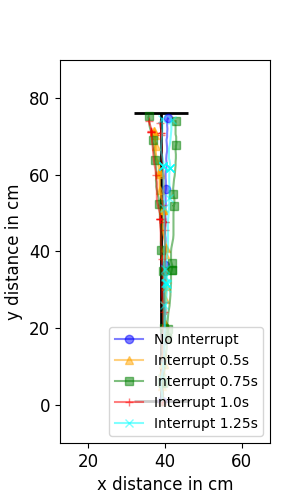
\includegraphics[width=\textwidth]{pics/straight_90.png}
		\caption{Target 90\%}
		\label{fig:stra_exp3}
	\end{subfigure}
	\caption{Straight movements for the different target duty cycles, the black horizontal line marks the 75\,cm endpoint.}
	\label{fig:straight_movements}
\end{figure}

\subsubsection{Movement Accuracy Metrics}

%The first metric is the length of movement, used to verify the accuracy between multiple iterations of the same calibrated speed and power interrupt combination.
%The second metric is used to describe deviation in path between the start and endpoint.
The robot has no reference to its surroundings to determine its absolute position and heading direction, i.e. no external feedback.
Therefore, only relative metrics are assumed to be valid.
For each measurement a reference line is computed between the first and last measured data point.
The Euclidean distance between the closest measurement and the reference line is computed.

\subsubsection{Straight Movement Results}

The results for the battery powered robot with and without artificial interrupts show that decreasing the on time, increases the maximum, average and standard deviation of the horizontal deviation, as seen in Table \ref{tab:straight_results}.
Increasing the speed does not have the same effect and no significant differences can be seen from the results.

The solar powered shows less horizontal deviation when compared to the battery powered robot.
This seems counter intuitive, but there is a suspicion that the additional weight of the solar panel has a big effect on the movement of the robot.
The weight of the solar panel is more than twice that of the battery, 5.2\,g and 2.1\,g respectively, and is more evenly distributed over the robot.
The robot without a battery or solar panel has a weight of 16.7\,g and therefore the weight of the solar panel can be considered significant when compared to the bare weight of the robot.

\begin{table}[t]
	\centering
	\caption{The Euclidean distance between the measurements and a reference line computed between start and end coordinates.}
	\label{tab:straight_results}
	\begin{tabular}{|l|l||l|l|l|}
		\hline
		Target (\%) & Interrupt (s) & Max (cm) & Mean (cm) & Std (cm)\\
		\hline \hline
		\multirow{4}{*}{40} & No interrupt & 0.86 & 0.36 & 0.16 \\
		%& 1.25 & 0.67 & 0.34 & 0.12 \\
		& 1.00 & 1.35 & 0.56 & 0.27 \\
		%& 0.75 & 1.04 & 0.60 & 0.27 \\
		& 0.50 & 0.86 & 0.44 & 0.22 \\
		& Solar & 0.50 & 0.25 & 1.35 \\
		\hline
		\multirow{4}{*}{65} & No interrupt & 0.52 & 0.25 & 0.12 \\
		%& 1.25 & 0.72 & 0.31 & 0.14 \\
		& 1.00 & 0.91 & 0.44 & 0.21 \\
		%& 0.75 & 1.44 & 0.80 & 0.35 \\
		& 0.50 & 2.15 & 1.17 & 0.54 \\
		& Solar & 0.41 & 0.17 & 1.05 \\
		\hline
		\multirow{4}{*}{90} & No interrupt & 0.54 & 0.28 & 0.13 \\
		%& 1.25 & 0.90 & 0.42 & 0.17 \\
		& 1.00 & 1.76 & 0.95 & 0.42 \\
		%& 0.75 & 1.88 & 0.88 & 0.37 \\
		& 0.50 & 2.18 & 1.09 & 0.61 \\
		& Solar & 0.30 & 0.15 & 0.69 \\
		\hline
	\end{tabular}
\end{table}

\subsection{Circular Movements}

The robot is programmed to make a circle with radius of 30\,cm with the predetermined speed and on times.
The results in Figure \ref{fig:circular_movements} show that for all measurements the robot is able perform the circular movement.
A clear difference in circle radius can be seen for each on time, as a result of an error between the actual and calibrated speeds.
The robot sometimes overshoots its final position.
It is expected to be caused by an error in integration of the angular velocity to obtain an angle.
The angle is used to determine if the movement target is reached.
Decreasing the power interrupt frequency is suspected to increases the integration error due to frequent accelerations from zero by the robot.
%Every time the robot starts a movement, the controller needs time to correct the robots heading.

\begin{figure}[h!]
	\centering
	\begin{subfigure}[b]{0.49\textwidth}
		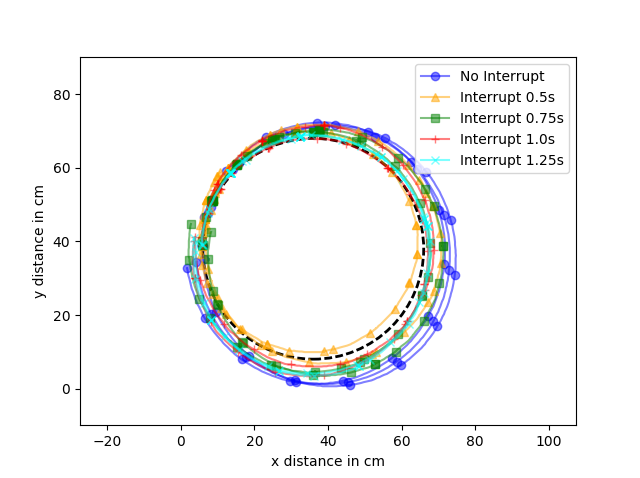
\includegraphics[width=\textwidth]{pics/circle_40.png}
		\caption{Target 40\%}
		\label{fig:circ_exp1}
	\end{subfigure}
	\begin{subfigure}[b]{0.49\textwidth}
		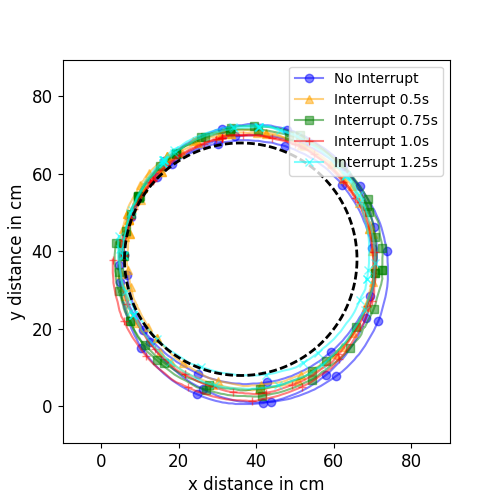
\includegraphics[width=\textwidth]{pics/circle_65.png}
		\caption{Target 65\%}
		\label{fig:circ_exp2}
	\end{subfigure}

	\begin{subfigure}[b]{0.49\textwidth}
		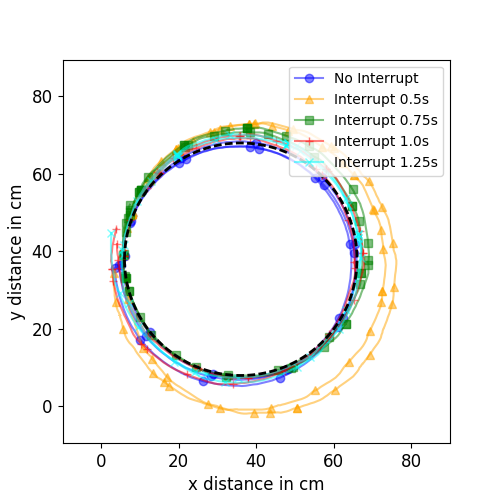
\includegraphics[width=\textwidth]{pics/circle_90.png}
		\caption{Target 90\%}
		\label{fig:circ_exp3}
	\end{subfigure}
	\caption{Circular movements for the different target duty cycles, the black dashed circle marks the programmed circle with a radius of 30\,cm.}
	\label{fig:circular_movements}
\end{figure}

\subsubsection{Movement Accuracy Metrics}

%The length of the movement is determined by summing the distance between points in the measurement data.
% two different metrics are used.
To determine the accuracy of the circular movement, a circle with varying radius is visually fitted to data of each movement.
The radius is different because calibrated speed varies with each target duty cycle and on time.
The Euclidean distance is computed between the reference circle and the measured circular movements.


\begin{table}[t]
	\centering
	\caption{The Euclidean distance between the measurements and a best fitting circle.}
	\label{tab:circular_results}
	\resizebox{\columnwidth}{!}{%
		\begin{tabular}{|l|l||l|l|l|l|}
			\hline
			Target (\%) & Interrupt (s) & Radius (cm) & Max (cm) & Mean (cm) & Std (cm)\\
			\hline \hline
			\multirow{4}{*}{40} & No interrupt & 34 & 4.30 & 1.30 & 0.67 \\
			%& 1.25 & 32 & 2.59 & 1.29 & 0.69 \\
			& 1.00 & 32 & 3.95 & 1.52 & 0.81 \\
			%& 0.75 & 33 & 4.07 & 1.21 & 0.82 \\
			& 0.50 & 32 & 6.08 & 1.85 & 1.30 \\
			& Solar & 32 & 1.93 & 0.89 & 0.46 \\
			\hline
			\multirow{4}{*}{65} & No interrupt & 34 & 3.03 & 1.2 & 0.67 \\
			%& 1.25 & 32 & 2.64 & 1.01 & 0.57 \\
			& 1.00 & 32 & 4.20 & 1.42 & 0.92 \\
			%& 0.75 & 33 & 2.89 & 1.11 & 0.73 \\
			& 0.50 & 32 & 1.86 & 0.79 & 0.34 \\
			& Solar & 31 & 1.93 & 0.88 & 0.4 \\
			\hline
			\multirow{4}{*}{90} & No interrupt & 30 & 2.37 & 0.9 & 0.45 \\
			%& 1.25 & 30 & 2.99 & 0.81 & 0.43 \\
			& 1.00 & 31 & 3.50 & 1.06 & 0.65 \\
			%& 0.75 & 31 & 2.12 & 0.71 & 0.41 \\
			& 0.50 & 35 & 4.53 & 1.69 & 1.23 \\
			& Solar & 31 & 2.10 & 0.88 & 0.37 \\
			\hline
		\end{tabular}
	}
\end{table}

\subsubsection{Circular Movement Results}
The average deviation from the reference circle reduces when the target duty cycle is increased, as seen from Table \ref{tab:circular_results}.
The additional speed is likely to provide more stability to the movement, since less interrupts are required to complete the circular movement, i.e. the controller is able to provide more direction.
The solar powered robot shows more stability when compared to the battery powered robot.
Which is expected to be a positive effect of the additional solar panel weight, as explained in the results of Section \ref{eval:straight_movements}.
